\chapter{密近双星}
\section{密近双星系统的引力}
如图\ref{fig:binary}所示,在双星系统中,引力等势面呈现为``8''字型,这个等势面被称为\textbf{洛希瓣},中间的交点为引力平衡点,被称为\textbf{拉格朗日点}。

\begin{figure}[hbt]
  \centering
  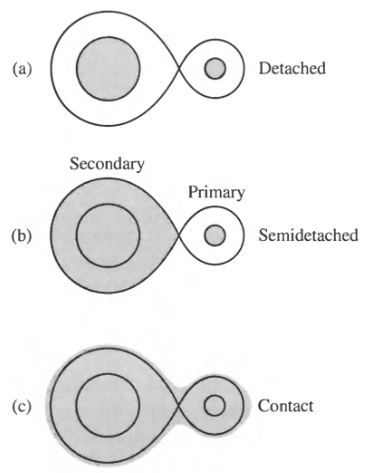
\includegraphics[width=6cm]{chapters/18/binary}
  \caption{双星系统的分类}
  \label{fig:binary}
\end{figure}

当两颗星距离足够远时,它们之间几乎不发生相互作用,属于\textbf{分离}形双星系统。

当两颗星足够近,且一颗恒星膨胀至洛希瓣时,由于引力的作用其性质也会变成泪滴状,并且拉格朗日点附近的物质一旦越过拉格朗日点,就会受另一颗星的引力作用而被吸引过去,这种属于\textbf{半分离}形双星系统。其中接受物质的恒星被称为\textbf{主星},失去物质的被称为\textbf{次星}。

如果两颗双星都充满了洛希瓣,那么它们之间就可以很容易地发生物质交换,这种属于\textbf{相接}形双星系统。

通过计算可以得到拉格朗日点当两星重点的距离分别为:
\begin{align}
  \ell_1 &=a\left[0.500-0.227\log_{10}\left({M_2\over M_1}\right)\right]\\[2mm]
  \ell_2 &=a\left[0.500+0.227\log_{10}\left({M_2\over M_1}\right)\right]
\end{align}

其中下标1代表主星,下标2代表次星。

\section{吸积}
对于半分离形双星系统,主星吸引次星越过拉格朗日点的物质的过程被称为\textbf{吸积},并会在周围形成\textbf{吸积盘},假设双星模型为两个交叠的圆,单位时间吸积质量的多少用\textbf{质量转移率(吸积率)}来描述:
\begin{equation}
  \dot M\approx \pi Rd\rho \sqrt{3kT\over m_H}
\end{equation}

其中$R$为洛希瓣半径,$d$为交叠的长度。

\section{双星系统的演化}
首先考虑两颗星初始是分离型双星系统,当一颗较小质量恒星演化为红巨星膨胀时,会填充洛希瓣,变成半分离形双星系统。随着主星的吸积,次星的质量会减小,引力会减弱,洛希瓣因此收缩,这会进一步增加吸积率,加快主星的吸积。

之后双星系统会被次星的物质所包围,变成相接双星系统,次星只剩下了简并核。双星在气体团中运动时会与气体摩擦,损失角动量,轨道会缩小,这可能会导致两颗星的并合,形成单星。

如果双星没有并合,反过来,轨道缩小也会导致洛希瓣缩小,原来的主星填满了洛希瓣,继而变成了次星,被反向吸积,但是因为现在的次星有较大的质量,吸积率会被维持在一个稳定的速率,最终变成两个轨道近密的双白矮星。其中一个质量较小、体积较大的白矮星会超出它的洛希瓣,然后分解在另一颗质量较大的白矮星周围形成吸积盘,如果主星吸积之后质量超过钱德拉塞卡极限,则会产生Ia型超新星爆发。

以上演化过程见图\ref{fig:binaryevolution},需要注意的是这只是一种设想,实际演化过程会受多种因素影响。

相接双星系统也可以分成多种种类,而很多是根据最早发现的相应的天体命名的:
\begin{itemize}
  \item 大陵五,两个一般恒星组成的半分离系统
  \item 猎犬座RS和天龙座BY,色球层活跃双星
  \item 大熊座W型相接双星,磁场活跃度很高
  \item 激变变星和类新星双星,白矮星和冷的M形次星
  \item 黑洞和中子星组成的X射线双星
  \item 御夫座ζ和仙王座VV,晚型超巨星和热的(一般为B星)伴星
  \item 共生双星,M型巨星被白矮星、亚矮星或低质量主序星吸积
  \item 钡和S光谱型星,白矮星和S光谱型(K型和M型之间)次星
  \item 共包层后双星,热白矮星和较冷次星
\end{itemize}

\begin{figure}[hbt]
  \centering
  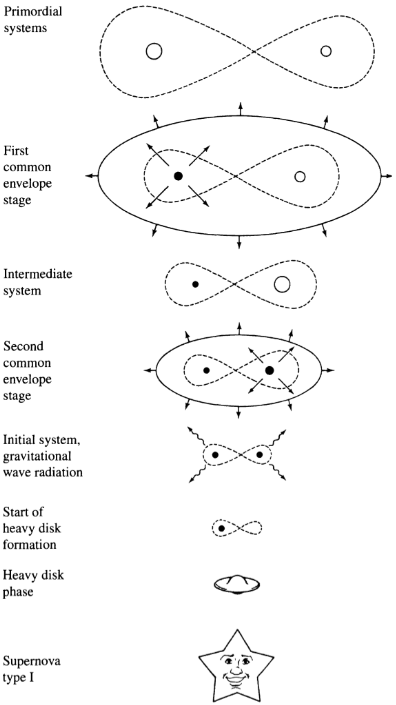
\includegraphics[width=9cm]{chapters/18/evolution}
  \caption{双星系统演化示意图}
  \label{fig:binaryevolution}
\end{figure}

\section{Ia型超新星}
前面描述到,主星白矮星在吸积次星白矮星分解后的物质,当质量达到钱德拉塞卡极限时,会产生Ia型超新星爆发,这是\textbf{超新星的一种产生模型}。\textbf{另一种模型}也可以是白矮星吸积正常恒星的物质,达到钱德拉塞卡极限后也会产生Ia型超新星。而这两种模型中,物质落在白矮星上产生超新星,会将白矮星也炸毁。

由于爆发时质量都为$1.4\,M_\odot$,爆发时的光度也就基本都相同,因此Ia型超新星可以作为标准烛光来测定距离。

\paragraph{毫秒脉冲星}
被认为产生于X射线双星中,但依旧可以分为两类:在大质量X射线双星中的毫秒脉冲星具有大质量的伴星(中子星),这类公转周期短且为偏心轨道;低质量X射线双星中的具有低质量伴星(白矮星),这类公转周期长且为圆轨道
